\documentclass[a4paper,12pt]{article}
\usepackage[utf8]{inputenc}
\usepackage[T1]{fontenc}
\usepackage[margin=25mm, footskip=15mm]{geometry}
\usepackage{amsmath}
\usepackage{graphicx}
\usepackage{caption}
\usepackage{floatpag}
\usepackage{pdflscape}
\usepackage{hyperref}

\title{%
  
\includegraphics[width=0.35\textwidth]{docs_bin/nobg-light-logo.png}\\[1em]
  \textbf{GreenBox} \\ System Documentation}
\author{
  Kolomiiets Ivan
  \and Plaster Desir\'{e}e Maria
  \and Fokuhl Robin-Niklas
  \and Kuca Rino
}
\date{\today}

\sloppy
\begin{document}

\maketitle
\tableofcontents

\newgeometry{margin=10mm, bottom=15mm, footskip=10mm}
\begin{landscape}
\thispagestyle{plain}
  \centering
  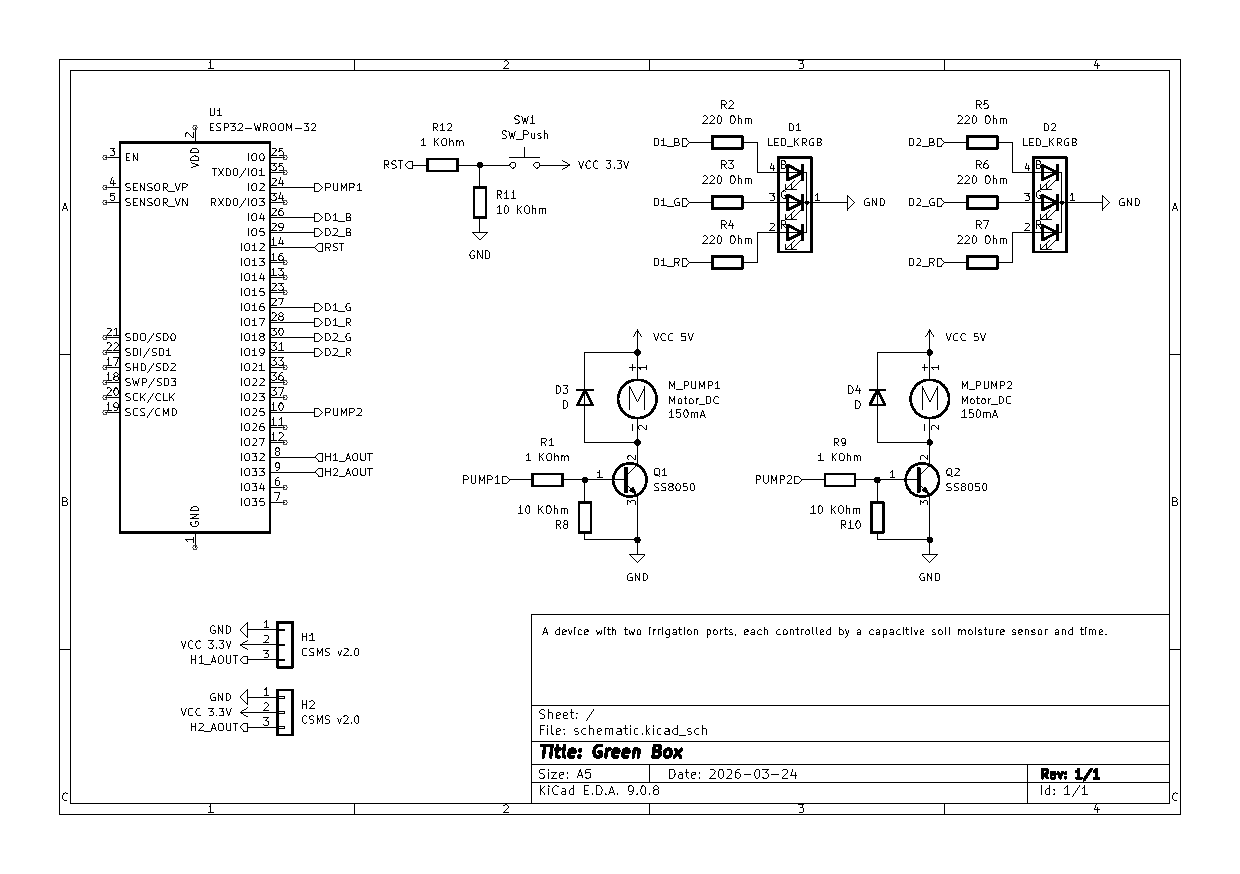
\includegraphics[width=\linewidth, height=0.96\textheight, keepaspectratio]{../schematic/green-box-schematic.pdf}
  \captionof{figure}{GreenBox PCB schematic (Rev~1/1, 2026-03-24).}
  \label{fig:schematic}
\end{landscape}
\restoregeometry

%% ---------------------------------------------------------------
\section{Global Sequence Overview}

This diagram shows the high-level lifecycle of a GreenBox device: power-on,
WiFi and MQTT broker configuration (Phase~1), device registration (Phase~2),
configuration protocol (Phase~3), watering event reporting (Phase~4), and user
data viewing (Phase~5). Each phase is documented in detail in a separate
diagram. See Figure~\ref{fig:global-sequence}.

%% ---------------------------------------------------------------
\section{System Architecture}

The GreenBox system follows a decoupled, broker-mediated architecture
(see Figure~\ref{fig:component}). The ESP32 device communicates exclusively
through an MQTT broker rather than directly with the application server. This
design was chosen for several reasons:

\begin{itemize}
  \item \textbf{Low overhead} --- MQTT's minimal packet format is well-suited
        for the ESP32's constrained memory and processing power. An HTTP-based
        approach would require maintaining a full TCP connection per request
        with significantly larger headers.
  \item \textbf{Persistent connection} --- a single MQTT session handles
        registration, configuration, and event reporting. The keep-alive
        mechanism (60\,s) detects disconnections faster than periodic HTTP
        polling.
  \item \textbf{Broker decoupling} --- the device and server are independent
        subscribers. The server can be restarted, scaled, or replaced without
        affecting connected devices. The broker queues messages during server
        downtime (with QoS~1 and persistent sessions).
  \item \textbf{Retained messages} --- MQTT's retain flag enables offline
        configuration delivery. When a device reconnects, it immediately
        receives the latest config without the server needing to know the
        device came online.
\end{itemize}

PostgreSQL was selected as the data store for the following reasons:
\begin{itemize}
  \item \textbf{Performance} --- advanced query planner, JSONB indexing, and
        BIGSERIAL primary keys handle unbounded time-series growth efficiently.
  \item \textbf{Open source} --- no licensing costs, large community, and
        transparent development.
  \item \textbf{High reliability and availability} --- ACID compliance,
        write-ahead logging, and mature replication support ensure data
        integrity even under unexpected failures.
  \item \textbf{Fully-featured DB and DBMS} --- native JSONB type allows
        storing the watering schedule (a variable-length array of
        time/duration pairs) without a separate join table, alongside
        constraints, triggers, and rich SQL support.
  \item \textbf{Cloud suitability} --- unlike embedded databases such as
        SQLite, PostgreSQL operates as a standalone server process, supporting
        concurrent access from multiple application instances, connection
        pooling, and managed cloud deployments (e.g.\ AWS RDS, GCP Cloud SQL).
\end{itemize}

The ESP32 runs a local web server (HTTP, port~80) solely for initial
provisioning. This server is active only during Phase~1 --- before the device
has internet connectivity --- and is destroyed once WiFi credentials are
confirmed.

%% ---------------------------------------------------------------
\section{Hardware}

The GreenBox PCB (Rev~1/1, KiCad~9.0.8) is built around an
ESP32-WROOM-32 module. The schematic is in \texttt{schematic/}. Key
peripherals:

\begin{itemize}
  \item \textbf{Humidity sensors} --- two CSMS~v2.0 capacitive soil moisture
        sensors (H1, H2), each providing an analog voltage on CH1\_AOUT /
        CH2\_AOUT (GPIO32, GPIO33). The firmware reads via ADC1 channels~4
        and~5 with 12-bit resolution and 12\,dB attenuation ($0$--$3.3$\,V
        range). Mapping: high ADC value = dry soil = low humidity\,\%;
        linear inverse: $\text{humidity} = 100 \times (1 - \text{raw}/4095)$\,\%.
  \item \textbf{RGB LEDs} --- two common-cathode LED\_KRGB (D1~=~Network,
        D2~=~Application), each with three 220\,$\Omega$ current-limiting
        resistors (R, G, B channels). Connected to six GPIO pins for
        independent GPIO digital control (on/off per channel, no dimming).
        Colors are binary R/G/B combinations: red~=~100, green~=~010,
        yellow~=~110, white~=~111, purple~=~101, blue~=~001, cyan~=~011.
  \item \textbf{Water pumps} --- two DC motors (150\,mA each), driven via
        SS8050 NPN transistors (Q1, Q2) with 1\,k$\Omega$ base resistors and
        10\,k$\Omega$ pulldowns. PUMP1 and PUMP2 on separate GPIO pins.
        Transistors are necessary because ESP32 GPIOs can only supply up to
        40\,mA, while each motor draws 150\,mA. Flyback diodes (D3, D4)
        across the motors protect against voltage spikes when the motors
        turn off. The 10\,k$\Omega$ pulldowns keep the transistors OFF
        while GPIOs are floating during boot.
  \item \textbf{Reset button} --- SW1 (push-button) with R12 (1\,k$\Omega$)
        in series and R11 (10\,k$\Omega$) pulldown. Connected to RST
        (GPIO12). Holding the button for 5\,s erases all NVS data and
        restarts the device, re-entering provisioning mode.
\end{itemize}

\subsection{GPIO Pin Assignments}

\begin{center}
\begin{tabular}{llll}
\hline
\textbf{Function} & \textbf{GPIO} & \textbf{Direction} & \textbf{Notes} \\
\hline
LED1 Red (D1)     & IO17 & Output & 220\,$\Omega$ to LED \\
LED1 Green (D1)   & IO16 & Output & 220\,$\Omega$ to LED \\
LED1 Blue (D1)    & IO4  & Output & 220\,$\Omega$ to LED \\
LED2 Red (D2)     & IO19 & Output & 220\,$\Omega$ to LED \\
LED2 Green (D2)   & IO18 & Output & 220\,$\Omega$ to LED \\
LED2 Blue (D2)    & IO5  & Output & 220\,$\Omega$ to LED \\
Pump 1            & IO2  & Output & SS8050 via 1\,k$\Omega$ \\
Pump 2            & IO25 & Output & SS8050 via 1\,k$\Omega$ \\
Humidity H1       & IO32 & ADC    & ADC1\_CH4 \\
Humidity H2       & IO33 & ADC    & ADC1\_CH5 \\
RST Button        & IO12 & Input  & Active high, 10\,k$\Omega$ pulldown \\
\hline
\end{tabular}
\end{center}

%% ---------------------------------------------------------------
\section{Firmware Architecture}

The ESP32 firmware is built with ESP-IDF~v6.0 using the framework's component
architecture. Each functional area is implemented as a separate component under
\texttt{gb-src/components/}, with explicit dependency declarations in
\texttt{CMakeLists.txt}:

\begin{itemize}
  \item \textbf{nvs\_manager} --- wraps NVS (Non-Volatile Storage) for storing
        and retrieving WiFi credentials (SSID, password), MQTT broker
        settings (host, port), and per-port watering configuration
        (config\_id, schedule JSON, humidity threshold, humidity duration).
        Namespace: \texttt{greenbox}.
  \item \textbf{led\_driver} --- controls the two RGB LEDs (D1, D2) via
        FreeRTOS timers for blinking patterns. Supports 13~distinct LED states
        covering all phases (steady, blinking, slow/fast blink
        in red, green, yellow, white, purple, blue, cyan).
  \item \textbf{wifi\_manager} --- manages WiFi in APSTA mode. On boot, the AP
        SSID is set to the device~ID (\texttt{GB-\{MAC\}}) and the password to
        the first 8~hex characters of the MAC address. Provides a blocking
        \texttt{try\_connect()} that waits for STA association or failure with
        a 15\,s timeout. Supports full stop/restart for hibernate.
  \item \textbf{web\_server} --- HTTP server for Phase~1 provisioning. Serves an
        embedded HTML form (\texttt{GET /}), a status endpoint
        (\texttt{GET /status}) for overheat polling, and a connect endpoint
        (\texttt{POST /connect}) that stores credentials in NVS, attempts WiFi
        connection, and verifies MQTT broker reachability via TCP probe before
        signaling success.
  \item \textbf{temp\_monitor} --- runs a FreeRTOS background task for overheat
        protection. During hibernate: stops WiFi and the web server entirely
        (LED~2 = purple). On exit: restarts both. Exposes
        \texttt{is\_hibernating()} for the web server to gate provisioning
        requests.
  \item \textbf{mqtt\_manager} --- implements Phases~2--4. For registration
        (Phase~2): connects via MQTT~5.0 (managed component
        \texttt{espressif/mqtt}) with device~ID as username and a hardcoded
        pre-shared key (\texttt{"greenbox"}) as password. Retries with
        exponential backoff (1\,s to 60\,s, max 10~attempts). After
        registration, the MQTT session stays open for Phases~3--4.
        For configuration (Phase~3): subscribes to \texttt{config/push},
        validates and stores configs in NVS per port, sends acknowledgment.
        Re-subscribes automatically on broker reconnect.
        For watering (Phase~4): runs schedule checks every 30\,s and
        humidity threshold checks every 60\,s via FreeRTOS timers.
        Watering runs in a dedicated FreeRTOS task (non-blocking queue)
        so MQTT keepalive is not disrupted during long pump cycles.
        Logs humidity sensor readings every 5\,s.
  \item \textbf{rst\_button} --- monitors GPIO12 by polling every 100\,ms.
        When the button is held HIGH for $\geq$5\,s, erases all NVS data
        and calls \texttt{esp\_restart()}, returning the device to
        provisioning mode on the next boot.
\end{itemize}

\subsection{Boot Flow}

On power-on, \texttt{app\_main} initializes NVS, WiFi (APSTA mode), the LED
driver, and the RST button monitor. It then reads saved WiFi credentials from
NVS. If credentials exist and the STA connection succeeds, provisioning is
skipped entirely. If no credentials are stored or the connection fails, the
device starts the provisioning AP and HTTP server as described in Phase~1.

After WiFi is connected (either path), the device synchronizes its clock via
SNTP from \texttt{pool.ntp.org} (up to 15 attempts, 1\,s timeout each).
Accurate time is required for schedule-triggered watering and for timestamps
in MQTT event payloads. The device then proceeds to Phase~2 registration
and, on success, enters the Phase~3/4 operational loop.

\subsection{Local MQTT Broker Setup}

For development, a Mosquitto~2 broker configuration is provided in
\texttt{broker/}:
\begin{itemize}
  \item \texttt{mosquitto.conf} --- plain TCP on port~1883, password
        authentication, ACL-based topic authorization.
  \item \texttt{passwd} --- password file (managed via \texttt{mosquitto\_passwd}).
        Each device authenticates with its device~ID as both username and
        client~ID, and a pre-shared key as password.
  \item \texttt{acl} --- uses Mosquitto's \texttt{pattern} directive with
        \texttt{\%u} (username) substitution to restrict each device to its own
        topic subtree. A \texttt{greenbox-server} admin user has full access.
  \item \texttt{docker-compose.yml} --- runs the broker standalone via
        \texttt{docker compose up} (for firmware-only testing).
\end{itemize}

\noindent A root-level \texttt{docker-compose.yml} runs the full stack:
Mosquitto broker, PostgreSQL~17 (initialized from
\texttt{server/sql/init.sql}), and the Python application server on
port~8000. Usage: \texttt{docker compose up --build} from the project root.

%% ---------------------------------------------------------------
\section{Database Schema}

The database uses three tables (see Figure~\ref{fig:er}):

\begin{itemize}
  \item \textbf{devices} --- one row per registered GreenBox. Populated during
        Phase~2 registration. The \texttt{status} column is
        \texttt{'active'} or \texttt{'inactive'}. The \texttt{last\_seen\_at}
        timestamp is updated on every registration, config ack, and watering
        event.
  \item \textbf{device\_configs} --- one row per configuration push, per port.
        This table is append-only: each new configuration creates a new row
        rather than overwriting the previous one, preserving a full audit trail
        of configuration changes. The \texttt{status} column tracks the
        lifecycle: \texttt{pending} (saved in DB) $\to$ \texttt{pushed}
        (published to MQTT, \texttt{pushed\_at} recorded) $\to$
        \texttt{applied} or \texttt{rejected} (device acknowledgment
        received, \texttt{acked\_at} recorded). Includes
        \texttt{humidity\_duration\_s} for humidity-triggered watering
        duration, independent of schedule slot durations.
  \item \textbf{watering\_events} --- one row per pump start/stop event.
        Uses BIGSERIAL because event volume grows linearly with time and number
        of devices. Each row stores both \texttt{device\_timestamp} (from
        device clock) and \texttt{received\_at} (server clock) to handle
        clock drift.
\end{itemize}

Configuration is stored per-port rather than as a monolithic device config.
Each GreenBox has two independent watering ports, and the user may update
one port's schedule without affecting the other. Using separate rows (rather
than two sets of columns in the \texttt{devices} table) also makes the schema
extensible if future hardware revisions add more ports.

The \texttt{watering\_schedule} column uses JSONB to store an array of
\texttt{\{time, duration\_s\}} objects. For an MVP this avoids the complexity
of a separate \texttt{schedule\_entries} table and join queries, while JSONB
operators still allow server-side filtering and validation.

%% ---------------------------------------------------------------
\section{MQTT Interface Definitions}

All MQTT messages follow a consistent topic naming convention
(see Figure~\ref{fig:mqtt-interfaces}):

\begin{center}
\texttt{greenbox/\{device\_id\}/\{domain\}/\{action\}}
\end{center}

\noindent where \texttt{domain} is one of \texttt{reg}, \texttt{config}, or
\texttt{event}, and \texttt{action} specifies the direction or type.

\textbf{QoS~1 (at-least-once)} is used throughout. Exactly-once (QoS~2) was
not chosen because it doubles the handshake overhead and the system already
handles duplicates: registration uses server-side upsert logic, configuration
uses the \texttt{config\_id} for idempotent application, and watering events
are idempotent inserts (duplicate timestamps on the same port are discarded).

The \texttt{retain} flag is set to \texttt{true} only on
\texttt{config/push}. This ensures that a device which was offline when the
user changed its configuration will receive the latest config immediately upon
reconnecting and re-subscribing. Watering events use \texttt{retain = false}
because they are time-series data: retaining only the most recent event would
be misleading, as the full history matters for analysis.

Every configuration and event message includes a \texttt{port} field (1 or 2)
to address the correct pump. This explicit port addressing keeps the topic
structure flat (one topic per message type) rather than embedding the port
number in the topic path, which would complicate wildcard subscriptions on the
server side.

%% ---------------------------------------------------------------
\section{Phase 1: WiFi + MQTT Broker Configuration}

On first boot (or when no saved credentials exist), the device creates a WiFi
hotspot with SSID equal to the device~ID (\texttt{GB-\{MAC\}}) and a password
derived from the first 8~hex characters of the MAC address. The AP runs on
channel~1 with WPA2-PSK authentication and supports up to 4~concurrent
stations. LED~1 blinks blue to indicate the provisioning AP is active and
waiting for a user connection.

The user connects to this hotspot, opens the on-device web interface at
\texttt{192.168.4.1}, and provides WiFi credentials (SSID, password) along
with the MQTT broker settings (host, port). Form fields are trimmed of
leading/trailing whitespace before storage. All parameters are persisted in
NVS.

The device attempts to connect to the specified WiFi network with a 15\,s
timeout. On success, it performs a TCP probe (5\,s timeout) to verify that the
MQTT broker is reachable at the given host and port before completing
provisioning. If the broker is unreachable, provisioning reports an error but
WiFi stays connected so the user can retry with a different broker address.

Overheat protection runs in parallel: if the device enters hibernate, LED~1
turns off, WiFi and the web server are shut down entirely. When temperature
normalizes, both are restarted and LED~1 resumes blue blinking.

On subsequent boots, saved credentials are tried automatically (LED~1 = red
blinking during the attempt). If the connection succeeds, provisioning is
skipped. See Figure~\ref{fig:phase1}.

%% ---------------------------------------------------------------
\section{Phase 2: Device Registration via MQTT}

After WiFi connectivity is established, the ESP32 registers itself with the
server through the MQTT broker (MQTT~5.0, plain TCP, port~1883 --- MVP, no
TLS). The device authenticates with its device~ID as both MQTT client~ID and
username, and a hardcoded pre-shared key (\texttt{"greenbox"}) as password.
The MQTT keep-alive is set to 60\,s.

The registration payload includes: \texttt{device\_id}, \texttt{mac\_address},
\texttt{firmware\_version} (hardcoded \texttt{"1.0.0"}),
\texttt{hardware\_revision} (hardcoded \texttt{"rev3"}), and
\texttt{uptime\_ms}. The server responds with a status and a config block
containing \texttt{telemetry\_interval\_s} and \texttt{ota\_check\_interval\_s}
(reserved for later use, not consumed by the MVP firmware).

The registration follows an exponential backoff retry loop (up to 10~attempts:
1, 2, 4, 8, 16, 32, 60, 60, 60, 60\,s). LED~2 indicates the failure type:

\begin{itemize}
  \item \textbf{Red fast blink} (150\,ms) --- connection error (DNS failure,
        MQTT auth rejected)
  \item \textbf{Red slow blink} (1\,s) --- TCP connection failed, subscribe
        or publish failed
  \item \textbf{White blinking} (500\,ms) --- server response timeout
        (no reply within 10\,s)
  \item \textbf{Red steady} --- server responded with ``rejected'' or max
        retries exhausted
  \item \textbf{Yellow blinking} (500\,ms) --- registration in progress
  \item \textbf{Green steady} --- registration successful
\end{itemize}

\noindent See Figure~\ref{fig:phase2}.

%% ---------------------------------------------------------------
\section{Phase 3: Configuration Protocol}

Once registered, the device subscribes to its configuration topic and awaits
instructions from the server (see Figure~\ref{fig:phase3}).

The configuration flow is initiated by the user through the web dashboard, not
by the device. The user selects a port (1 or 2) and optionally sets:

\begin{itemize}
  \item \textbf{Watering schedule} --- daily time slots, each with a
        UTC time (HH:MM) and duration in seconds. Empty = no scheduled
        watering. The MVP firmware stores at most 8~slots per port; any
        slots beyond 8 are silently dropped.
  \item \textbf{Humidity threshold} (\texttt{humidity\_threshold\_pct}, 0--100)
        --- the soil moisture level below which watering triggers
        automatically. Set to 0 to disable humidity-triggered watering.
  \item \textbf{Humidity duration} (\texttt{humidity\_duration\_s}) --- the
        pump run time in seconds when humidity triggers watering. Independent
        of schedule slot durations. Set to 0 to disable.
\end{itemize}

\noindent All fields are optional; empty schedule and zero thresholds disable
the respective trigger. The web frontend sends a POST request to the server,
which validates the input, stores it in \texttt{device\_configs} with
\texttt{status = pending}, and publishes it to the MQTT broker with
\texttt{retain = true}.

Retained messages are central to this design. If the device is online, it
receives the config immediately. If it is offline (powered down, WiFi lost),
the broker stores the retained message and delivers it the moment the device
reconnects and re-subscribes. This eliminates the need for the server to track
device online/offline state or implement a push-retry mechanism.

Each configuration carries a unique \texttt{config\_id}. The device stores the
last applied \texttt{config\_id} per port in NVS. When the same
\texttt{config\_id} arrives again --- due to QoS~1 redelivery or the retained
message on reconnect --- the device re-sends the acknowledgment but does not
re-apply the configuration. This provides idempotency without requiring
exactly-once delivery.

The device validates all fields locally before applying. A rejected
configuration triggers LED~2 = white steady for 10\,s, then returns to green.
The acknowledgment includes \texttt{status = "rejected"} and a \texttt{reason}
string. Defined rejection reasons:

\begin{itemize}
  \item \texttt{"missing\_fields"} --- required fields (\texttt{config\_id},
        \texttt{port}) absent from payload.
  \item \texttt{"invalid\_values"} --- \texttt{port} not in $\{1, 2\}$ or
        \texttt{humidity\_threshold\_pct} outside 0--100.
\end{itemize}

\noindent In the MVP, the server extracts only \texttt{config\_id} and
\texttt{status} from the ack message. Other fields (\texttt{timestamp},
\texttt{port}, \texttt{reason}) are sent by the device for later use but
are not stored.

Watering schedule times are specified in UTC. The ESP32 synchronizes its
clock via SNTP (\texttt{pool.ntp.org}) after WiFi connection, not from the
server's \texttt{server\_time} field.

Configuration is stored in NVS keyed by port number (config\_id, schedule
JSON, humidity threshold, humidity duration), ensuring it survives device
reboots without requiring a re-push from the server. The status lifecycle
is tracked with separate timestamps: \texttt{pushed\_at} (when the MQTT
message was published) and \texttt{acked\_at} (when the device acknowledged).

%% ---------------------------------------------------------------
\section{Phase 4: Watering Event Reporting}

The GreenBox reports every pump activation and deactivation as a watering
event (see Figure~\ref{fig:phase4}).

Two triggers can start a watering cycle:

\begin{enumerate}
  \item \textbf{Schedule trigger} --- a FreeRTOS timer checks every 30\,s
        whether the current UTC hour:minute matches any configured slot.
        A same-minute deduplication guard prevents re-triggering within the
        same minute. When matched, the device reads the humidity sensor for
        that port, activates the pump GPIO (HIGH), and runs for the slot's
        configured \texttt{duration\_s}.
  \item \textbf{Humidity trigger} --- a separate timer checks every 60\,s
        whether the humidity reading is below
        \texttt{humidity\_threshold\_pct}. If so, the pump runs for
        \texttt{humidity\_duration\_s} (independent of schedule durations).
        Both \texttt{humidity\_threshold\_pct} and
        \texttt{humidity\_duration\_s} must be $>0$ for this trigger to be
        active.
\end{enumerate}

\noindent Watering runs in a dedicated FreeRTOS task that reads from a queue.
Timer callbacks post commands to the queue without blocking, so the MQTT
keep-alive (60\,s) is never disrupted during long pump cycles. LED~2 =
cyan blinking while a pump is active, green steady when idle.

In addition to threshold checks, the device logs humidity readings from both
sensors every 5\,s at INFO level for diagnostic purposes.

Each event payload includes a \texttt{trigger} field (\texttt{"schedule"} or
\texttt{"humidity"}) and real UTC timestamps from the SNTP-synchronized
clock. Start events include \texttt{humidity\_at\_start\_pct} and
\texttt{planned\_duration\_s}; stop events include
\texttt{humidity\_at\_stop\_pct}, \texttt{actual\_duration\_s}, and
\texttt{stop\_reason}. The \texttt{stop\_reason} field enables post-hoc
analysis: \texttt{duration\_complete} indicates a normal cycle, and
\texttt{error} indicates a pump fault or sensor failure.

Events are published immediately upon pump start and stop --- they are not
batched or deferred. A user watching the dashboard should see the pump status
change within seconds.

The server subscribes to \texttt{greenbox/+/event/watering} (max QoS~1) using
a wildcard, which scales to any number of devices without per-device
subscription management. Each event is stored with both a
\texttt{device\_timestamp} (from the device's clock) and a
\texttt{received\_at} (server wall clock) to handle clock drift. The server
also updates the device's \texttt{last\_seen\_at} on every event received.

%% ---------------------------------------------------------------
\section{Phase 5: User Data Viewing}

The web frontend provides a dashboard for monitoring device status,
watering history, and configuration (see Figure~\ref{fig:phase5}).

The application server (Python / FastAPI) runs an MQTT background task that
subscribes to three wildcard topics (max QoS~1, matching the QoS devices
publish with):

\begin{itemize}
  \item \texttt{greenbox/+/reg/request} --- device registrations
  \item \texttt{greenbox/+/config/ack} --- configuration acknowledgments
  \item \texttt{greenbox/+/event/watering} --- watering events
\end{itemize}

\noindent The MQTT client reconnects automatically with a 5\,s delay if the
broker restarts.

The REST API is the sole interface between the web frontend and the server.
The frontend never communicates with the MQTT broker directly.

\subsection{REST API Endpoints}

\begin{center}
\begin{tabular}{lll}
\hline
\textbf{Method} & \textbf{Path} & \textbf{Description} \\
\hline
GET  & \texttt{/api/devices}                       & List all devices \\
GET  & \texttt{/api/devices/\{id\}}                & Device detail + configs + events \\
POST & \texttt{/api/devices/\{id\}/config}          & Push config to device \\
GET  & \texttt{/api/devices/\{id\}/config?port=N}   & Latest config for port \\
GET  & \texttt{/api/devices/\{id\}/watering}         & Watering history \\
\hline
\end{tabular}
\end{center}

\noindent The watering history endpoint accepts query parameters:
\texttt{port} (1 or 2), \texttt{from} and \texttt{to} (ISO~8601 timestamps),
and \texttt{limit} (1--200, default 50).

The device detail endpoint returns the latest configuration per port
(using PostgreSQL \texttt{DISTINCT ON (port) ... ORDER BY created\_at DESC}),
regardless of config status. The device detail page auto-refreshes every
10\,s.

The configuration update endpoint
(\texttt{POST /api/devices/\{device\_id\}/config}) returns immediately with
\texttt{status = pushed}, not \texttt{applied}. The actual application
happens asynchronously through the Phase~3 MQTT flow.

\subsection{Web UI}

The server renders two HTML pages via Jinja2 templates:

\begin{itemize}
  \item \texttt{GET /} --- device list (device~ID, status, firmware, last
        seen).
  \item \texttt{GET /devices/\{id\}} --- device detail with info card,
        per-port config panels (current config display + push form), and
        recent watering events table. The config push form accepts schedule
        lines (HH:MM duration\_s), humidity threshold (\%), and humidity
        duration (s); all fields are optional.
\end{itemize}

%% ---------------------------------------------------------------
\section{LED State Diagram}

The GreenBox uses two RGB LEDs for visual status indication
(see Figure~\ref{fig:led-states}):

\begin{itemize}
  \item \textbf{LED~1 (Network Status)} --- indicates WiFi connectivity state.
        Blue blinking = provisioning AP active; red blinking = connecting;
        green steady = connected; red steady = credentials rejected.
  \item \textbf{LED~2 (Application Status)} --- indicates registration
        progress, configuration activity, watering status, overheat
        protection, and general operational state.
\end{itemize}

\noindent Blink periods:

\begin{center}
\begin{tabular}{ll}
\hline
\textbf{State} & \textbf{Period} \\
\hline
Red blinking (normal)   & 500\,ms \\
Red slow blink          & 1000\,ms \\
Red fast blink          & 150\,ms \\
Yellow blinking         & 500\,ms \\
White blinking          & 500\,ms \\
Blue blinking           & 500\,ms \\
Cyan blinking           & 500\,ms \\
\hline
\end{tabular}
\end{center}

%% ===============================================================
\appendix
\newpage
\section{Diagrams}

\begin{figure}[ht]
\thisfloatpagestyle{plain}
  \centering
  \includegraphics[width=\textwidth, height=\textheight, keepaspectratio]{docs_bin/global-sequence.png}
  \caption{GreenBox global sequence --- top-level orchestration.}
  \label{fig:global-sequence}
\end{figure}

\newgeometry{margin=10mm, bottom=20mm, footskip=15mm}

\begin{figure}[p]
\thisfloatpagestyle{plain}
  \centering
  \includegraphics[width=\textwidth, height=\textheight, keepaspectratio]{docs_bin/component-diagram.png}
  \caption{System component diagram --- architecture overview.}
  \label{fig:component}
\end{figure}

\begin{figure}[p]
\thisfloatpagestyle{plain}
  \centering
  \includegraphics[width=\textwidth, height=\textheight, keepaspectratio]{docs_bin/er-diagram.png}
  \caption{Entity relationship diagram --- full database schema.}
  \label{fig:er}
\end{figure}

\newgeometry{margin=10mm, bottom=15mm, footskip=10mm}
\begin{landscape}
\thispagestyle{plain}
  \vspace*{\fill}
  \centering
  \includegraphics[width=\linewidth, height=0.90\textheight, keepaspectratio]{docs_bin/mqtt-interfaces.png}
  \captionof{figure}{MQTT message interface definitions.}
  \label{fig:mqtt-interfaces}
  \vspace*{\fill}
\end{landscape}
\restoregeometry

\begin{figure}[p]
\thisfloatpagestyle{plain}
  \centering
  \includegraphics[width=\textwidth, height=\textheight, keepaspectratio]{docs_bin/phase1-wifi-setup.png}
  \caption{Phase~1 --- WiFi and MQTT broker configuration sequence.}
  \label{fig:phase1}
\end{figure}

\begin{figure}[p]
\thisfloatpagestyle{plain}
  \centering
  \includegraphics[width=\textwidth, height=\textheight, keepaspectratio]{docs_bin/phase2-mqtt-registration.png}
  \caption{Phase~2 --- MQTT registration sequence.}
  \label{fig:phase2}
\end{figure}

\begin{figure}[p]
\thisfloatpagestyle{plain}
  \centering
  \includegraphics[width=\textwidth, height=\textheight, keepaspectratio]{docs_bin/phase3-config-protocol.png}
  \caption{Phase~3 --- Configuration protocol sequence.}
  \label{fig:phase3}
\end{figure}

\begin{figure}[p]
\thisfloatpagestyle{plain}
  \centering
  \includegraphics[width=\textwidth, height=\textheight, keepaspectratio]{docs_bin/phase4-watering-events.png}
  \caption{Phase~4 --- Watering event reporting sequence.}
  \label{fig:phase4}
\end{figure}

\begin{figure}[p]
\thisfloatpagestyle{plain}
  \centering
  \includegraphics[width=\textwidth, height=\textheight, keepaspectratio]{docs_bin/phase5-user-data-viewing.png}
  \caption{Phase~5 --- User data viewing sequence.}
  \label{fig:phase5}
\end{figure}

\begin{figure}[p]
\thisfloatpagestyle{plain}
  \centering
  \includegraphics[width=\textwidth, height=\textheight, keepaspectratio]{docs_bin/led-states.png}
  \caption{RGB LED state diagram --- LED~1 (Network) and LED~2 (Application).}
  \label{fig:led-states}
\end{figure}

\restoregeometry

\end{document}
